\documentclass[11pt,a4paper]{article}

\usepackage{amsmath} %for mathemathic formulas
\usepackage{amssymb}
\usepackage[ngerman]{babel} %for the german language by the spellling reform (without the package the date would look like April 20, 2020)
\usepackage{enumitem} %for enumeration surrounding 
\usepackage{graphicx} %for pictures
\usepackage{siunitx}
\usepackage{float}

\title{Blatt 9}
\date{\today}
\author{Hannah Rotgeri \and Lena Olbrich}

\begin{document}
	\maketitle
	
	\section{Aufgabe 18}


	\begin{itemize}
		\item[b)] 
			Der erreichte Wert liegt bei 0,844.
		
		\item[c)]
			 Ein "roc auc score" von 0,5 würde bedeuten, dass richtige und falsche Einordung gleichwahrscheinlich ist.
			 1 würde bedeuten, dass jedes Ereignis richtig zugewiesen wird.

		\item[d)]
			 Die Genauigkeit steigt mit zunehmender Sensitivität,
			 mehr Werte richtig erkannt werden.
			 Die Sensitivität sinkt jedoch, da auch mehr positive Ereignisse verworfen werden.
		   
			\begin{figure}[H]
				\centering
				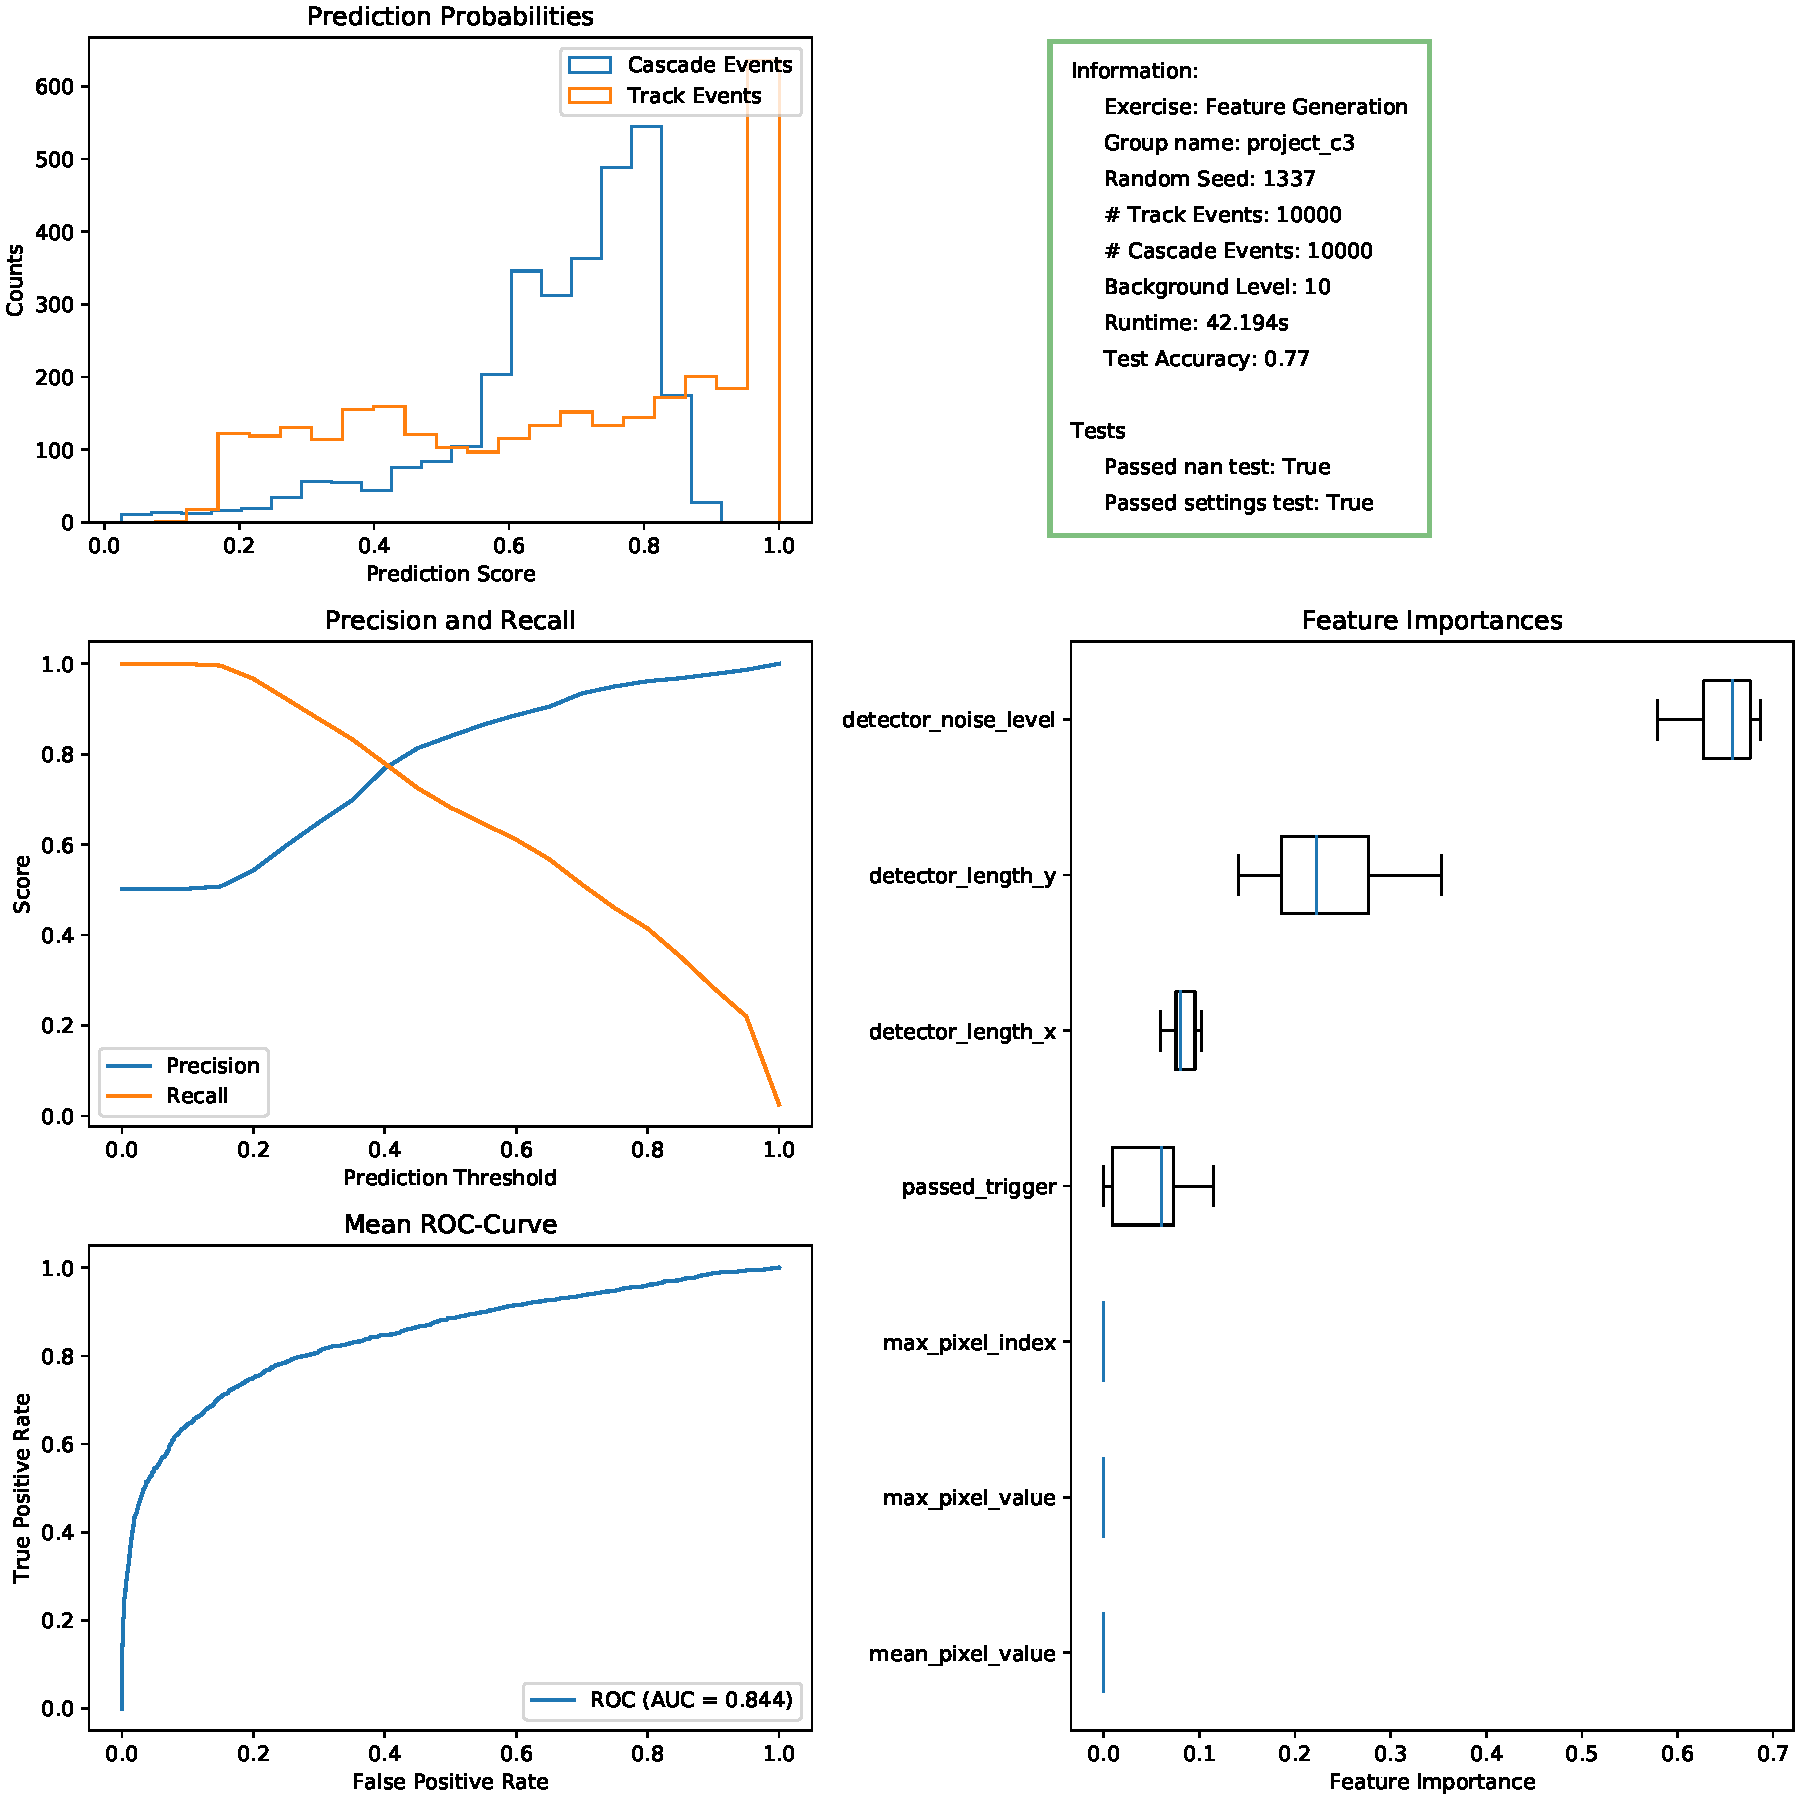
\includegraphics[width=\textwidth]{feature_generation.pdf}
			\end{figure} 

	\end{itemize}

	\section{Aufgabe 19}
	Diese Aufgabe konnten wir leider aus zeitlichen Gründen nicht bearbeiten.

\end{document}